\documentclass[14pt]{beamer}
\usetheme{EastLansing}
\usecolortheme{spruce}

\usepackage{xcolor}
\usepackage{listings}
\usepackage{courier}
\usepackage{graphicx}
\usepackage{amsmath}
\usepackage{algorithm2e}
\usepackage{multicol}

% https://tex.stackexchange.com/questions/42619/x-mark-to-match-checkmark
\usepackage{pifont}% http://ctan.org/pkg/pifont

\usefonttheme[onlymath]{serif}

\definecolor{mGreen}{rgb}{0,0.6,0}
\definecolor{mGray}{rgb}{0.5,0.5,0.5}
\definecolor{mPurple}{rgb}{0.8,0,0.82}
\definecolor{backgroundColour}{rgb}{0.95,0.95,0.92}
\definecolor{lightBlue}{rgb}{0.1, 0.1, 0.8}

\newcommand\red[1]{{\color{red} #1}}
\newcommand\green[1]{{\color{green} #1}}
\newcommand\blue[1]{{\color{blue} #1}}

\newcommand{\cmark}{\ding{51}}%
\newcommand{\xmark}{\ding{55}}%

\lstdefinestyle{CStyle}{
    backgroundcolor=\color{backgroundColour},   
    commentstyle=\color{mGreen},
    keywordstyle=\color{magenta},
    numberstyle=\tiny\color{mGray},
    stringstyle=\color{mPurple},
    basicstyle=\footnotesize,
    breakatwhitespace=false,         
    breaklines=true,                 
    captionpos=b,                    
    keepspaces=true,                 
    numbers=left,                    
    numbersep=5pt,                  
    showspaces=false,                
    showstringspaces=false,
    showtabs=false,                  
    tabsize=2,
    language=C
}
\lstdefinestyle{pseudo}{
        basicstyle=\ttfamily\footnotesize,
        keywordstyle=\color{lightBlue},
        morekeywords={BEGIN,END,IF,ELSE,ENDIF,ELSEIF,PRINT,WHILE,RETURN,ENDWHILE,DO,FOR,TO,IN,ENDFOR,BREAK,INPUT},
        morecomment=[l]{//},
        commentstyle=\color{mGreen}
}

\lstset{basicstyle=\footnotesize\ttfamily,breaklines=true}
\lstset{framextopmargin=50pt,tabsize=2}

\title{ENGG1003 - Monday Week 2}
\subtitle{First steps: libraries \& modules, plotting and printing}
\author{Steve Weller}
\institute{University of Newcastle}
\date{\today}

\begin{document}
\titlepage

%==============================================================

\begin{frame}[fragile]
\frametitle{Lecture overview}
\begin{enumerate}
\item Python program with a library function \red{\S1.3}
	\begin{itemize}
		\item principles
		\item live demo
	\end{itemize}
\item importing from modules and packages \red{\S1.4}
		\begin{itemize}
		\item principles
		\item live demo
	\end{itemize}
	
\item simple plotting \red{\S1.5} 
	\begin{itemize}
			\item principles
		\item live demo
	\end{itemize}
	
\item plotting and printing \red{\S1.6}
	\begin{itemize}
	\item principles
	\item live demo
	\end{itemize}
\end{enumerate}

%\begin{center}
%\texttt{https://link.springer.com/book/10.1007\%2F978-3-030-16877-3}
%\end{center}
\end{frame}

%==============================================================

\begin{frame}[fragile]
\frametitle{$1)$ Python program with a library function}
\begin{itemize}
\item describe the problem
\item simple diagram: $x, y, \theta$
\item maybe a ball?
\item algorithm is $\tan^{-1}$
\end{itemize}
\end{frame}

%==============================================================

\begin{frame}[fragile]
\frametitle{The program}

% screen grab of code from p.~12 text
\begin{figure}[ht]
	\centering
	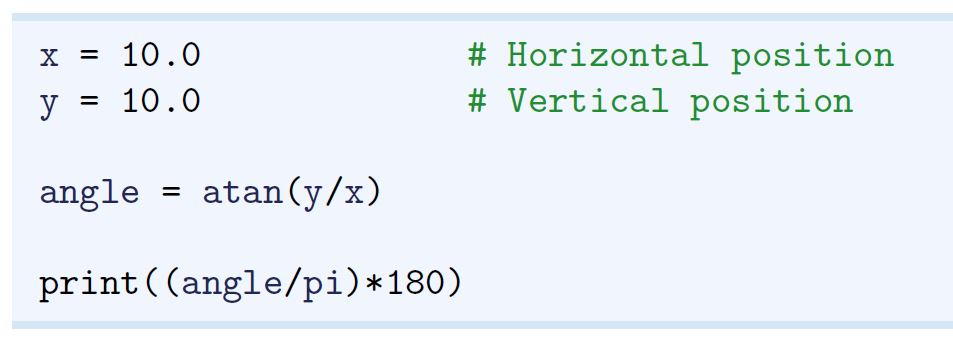
\includegraphics[width=\textwidth]{figures/LLp12}
\end{figure}

\begin{center}
\texttt{ball\_angle\_first\_try.py}
\end{center}

\end{frame}

%==============================================================

\begin{frame}[fragile]
\frametitle{First use of a Python function}
\begin{itemize}
\item first use of a \red{\emph{function}}, in this case \texttt{atan}
\item \red{\emph{argument}}
\item \red{\emph{return value}}
\end{itemize}

\end{frame}

%==============================================================

\begin{frame}[fragile]
\frametitle{Math review: radians and degrees}
\begin{itemize}
\item Python's \texttt{atan} returns value in radians
\item $\times \frac{180}{\pi}$ to get answer in degrees
\end{itemize}
\end{frame}

%==============================================================

\begin{frame}[fragile]
\frametitle{Running the program}
\begin{itemize}
\item screen grab from PyCharm -- error message
\end{itemize}
\end{frame}

%==============================================================

\begin{frame}[fragile]
\frametitle{Python standard library and import}
\begin{itemize}
\item Python has plenty of functionality ``built-in''
\item LOTS more can be \red{\emph{imported}}
\item \texttt{atan} and other trigonometric functions not built in
\item to activate that functionality, must explicitly import
\item \texttt{atan} function is grouped together with many other mathematical functions in a \red{\emph{library module}}  called \texttt{math}
\end{itemize}

% screen grab of code from p.~13 text
\begin{figure}[ht]
	\centering
	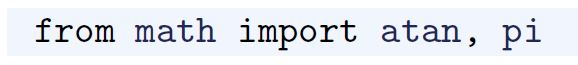
\includegraphics[width=0.6\textwidth]{figures/LLp13a}
\end{figure}

\end{frame}

%==============================================================

\begin{frame}[fragile]
\frametitle{The program: second attempt}

% screen grab of code from p.~13 text
\begin{figure}[ht]
	\centering
	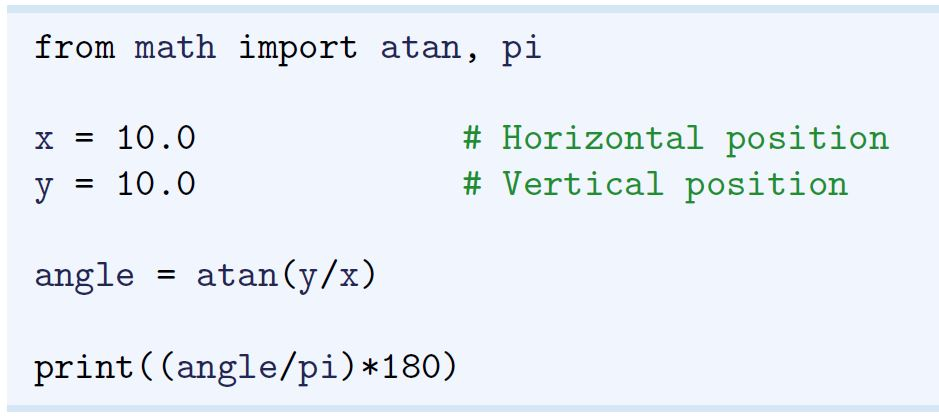
\includegraphics[width=0.9\textwidth]{figures/LLp13b}
\end{figure}
\begin{center}
\texttt{ball\_angle.py}
\end{center}
\begin{itemize}
\item script correctly produces $45.0$ as output
\item live demo in PyCharm shortly
\end{itemize}

\end{frame}

%==============================================================

\begin{frame}[fragile]
\frametitle{Another way of importing}
\begin{itemize}
\item use the import statement import math, but require \texttt{atan} and \texttt{pi} to be \red{\emph{prefixed}} with math
\item both techniques are commonly used and are the two basic ways of importing library code in Python
%\item Importing code is an evident part of Python programming, so we better shed some more light on it
\end{itemize}
\begin{figure}[ht]
	\centering
	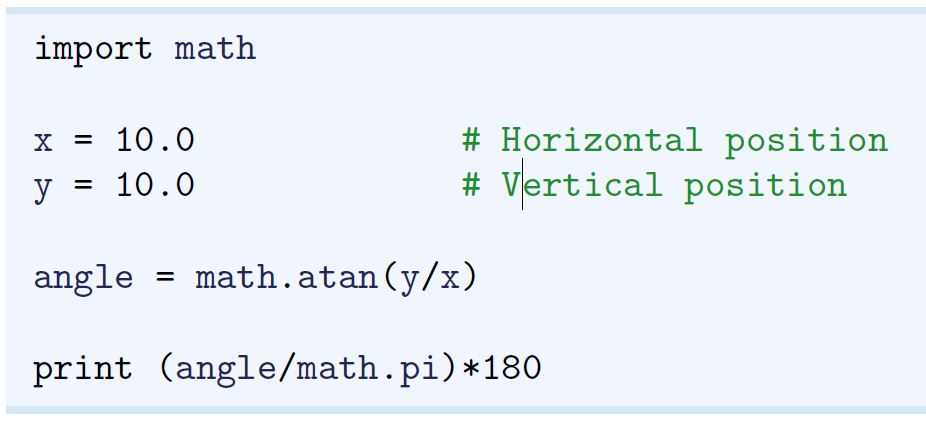
\includegraphics[width=0.7\textwidth]{figures/LLp14}
\end{figure}
\vspace*{-5mm}
\begin{center}
\texttt{ball\_angle\_prefix.py}
\end{center}

\end{frame}

%==============================================================

\begin{frame}[fragile]
\frametitle{Live demo of Python program with a library function}

\end{frame}

%==============================================================

\begin{frame}[fragile]
\frametitle{$2)$ Importing from modules and packages}

motivation and context

%At first, it may seem cumbersome to have code in different libraries, since it means
%you have to know (or find out) what resides in which library.10 Also, there are
%many libraries around in addition to the Python standard library itself. To your
%comfort, you come a long way with just a few libraries, and for easy reference, the
%handful of libraries used in this book is listed below (Sect. 1.4.5). Having everything
%available at any time would be convenient, but this would also mean that computer
%memory would be filled with a lot of unused information, causing less memory to be
%available for computations on big data. Python has so many libraries, with so much
%functionality, that importing what is needed is indeed a very sensible strategy.

\begin{itemize}
\item[(a)] importing for use \textbf{\emph{without}} prefix %, eg: \texttt{ball\_angle.py}

\item[(b)] importing for use \textbf{\emph{with}} prefix %, eg: \texttt{ball\_angle\_prefix.py}
\end{itemize}

\end{frame}

%==============================================================

\begin{frame}[fragile]
\frametitle{Importing for use \emph{without} prefix}

% screen grab of code from p.~13 text
\begin{figure}[ht]
	\centering
	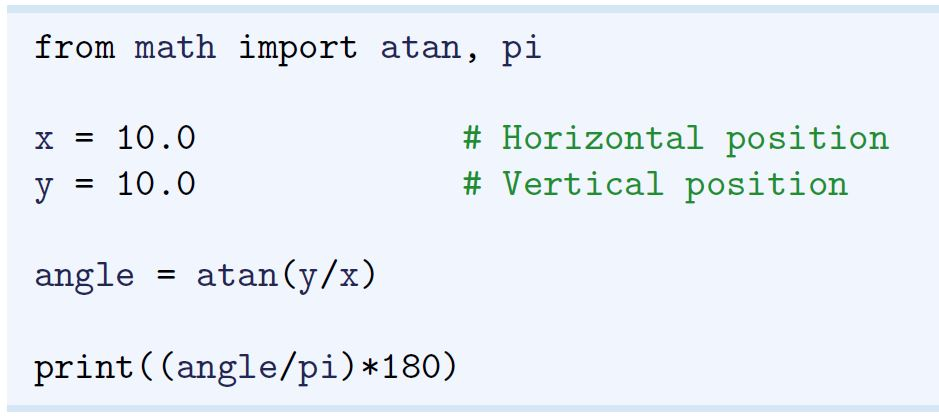
\includegraphics[width=0.8\textwidth]{figures/LLp13b}
\end{figure}
\begin{itemize}
\item[\green{\cmark}] Python code is easier to read
\item[\red{\xmark}] allows name conflicts!
\end{itemize}

%\cmark

\end{frame}

%==============================================================

\begin{frame}[fragile]
\frametitle{Name conflicts}
\begin{itemize}
\item explain the basic idea
\item do \emph{not} explain example from text, which is too complicated
\item will show an example shortly
\end{itemize}

\end{frame}

%==============================================================

\begin{frame}[fragile]
\frametitle{Importing for use \emph{with} prefix}

% screen grab of code from p14 text
\begin{figure}[ht]
	\centering
	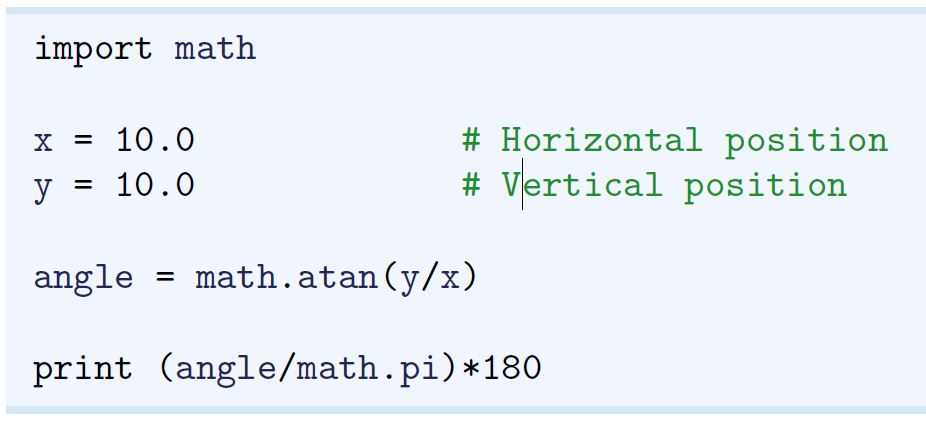
\includegraphics[width=0.8\textwidth]{figures/LLp14}
\end{figure}
\begin{itemize}
\item[\red{\xmark}] Python code is a little harder for humans to read
\item[\green{\cmark}\green{\cmark}] eliminates name conflicts!
\item \textbf{import with prefix is the standard and safer and preferred method of importing}
\end{itemize}

\end{frame}

%==============================================================

\begin{frame}[fragile]
\frametitle{Avoiding name conflict using prefixes}

% screen grab of code from p17 text
\begin{figure}[ht]
	\centering
	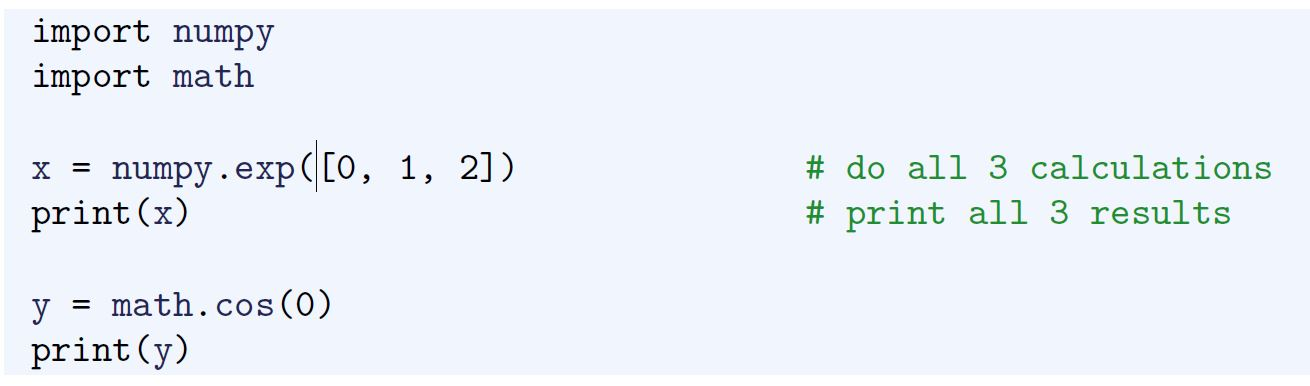
\includegraphics[width=0.8\textwidth]{figures/LLp17}
\end{figure}
\begin{itemize}
	\item \texttt{numpy} library includes an \texttt{exp} function
	\begin{itemize}
		\item math review:~exponential function $e^{z} =$~\texttt{exp(z)}
	\end{itemize}
	\item \texttt{math} library also includes an \texttt{exp} function---with a different implementation!
	\item[\green{\cmark}] \textbf{prefixes make clear which \texttt{exp} to use}
\end{itemize}

\end{frame}

%==============================================================

\begin{frame}[fragile]
\frametitle{Imports with name change}

% screen grab of code from p18 text
\begin{figure}[ht]
	\centering
	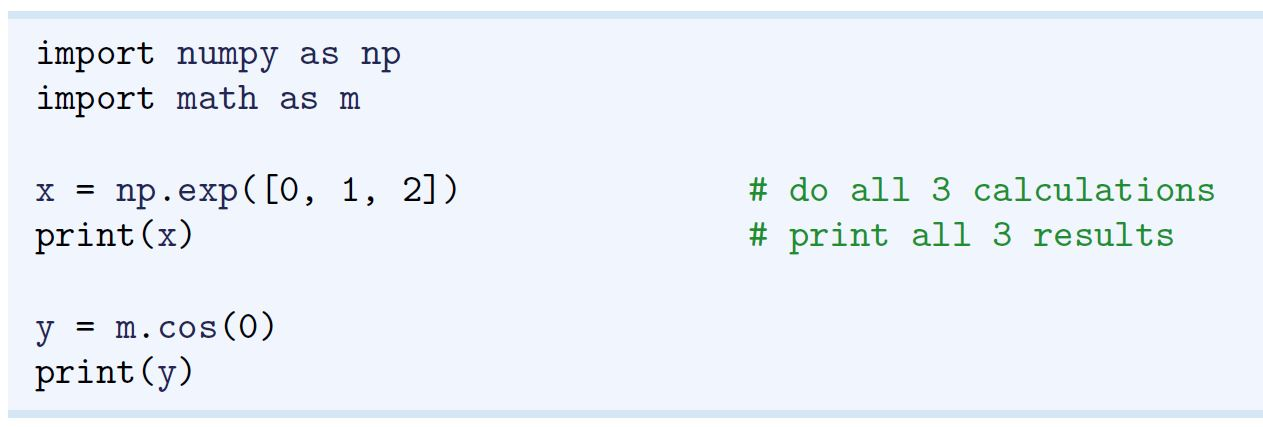
\includegraphics[width=0.9\textwidth]{figures/LLp18}
\end{figure}
\vspace*{-8mm}
\begin{itemize}
\item using \red{as}, \texttt{numpy} name becomes \texttt{np} 
\item similar for \texttt{math} and \texttt{m}
\item[\green{\cmark}] Python code is easy to read
\item[\green{\cmark}\green{\cmark}] eliminates name conflicts
\end{itemize}

\end{frame}

%%==============================================================
%
%\begin{frame}[fragile]
%\frametitle{Importing from packages}
%\begin{itemize}
%\item xxx
%\end{itemize}
%
%\end{frame}
%
%%==============================================================
%
%\begin{frame}[fragile]
%\frametitle{}
%\begin{itemize}
%\item xxx
%\end{itemize}
%
%\end{frame}

%%==============================================================
%
%\begin{frame}[fragile]
%\frametitle{}
%\begin{itemize}
%\item xxx
%\end{itemize}
%
%\end{frame}

%==============================================================

\begin{frame}[fragile]
%\frametitle{Main modules \& packages used in ENGG1003}
\frametitle{Main modules used in ENGG1003}
\begin{itemize}
\item \texttt{math}---description
\item \texttt{numpy}---description
\item \texttt{matplotlib}---description
%\item \texttt{random}---description
%\item \texttt{sympy}---description
%\item \texttt{timeit}---description
%\item \texttt{sys}---description
\end{itemize}

%math—see, e.g., ball_angle.py, Sect. 1.3.
%• numpy—see, e.g., check_functions.py above.
%• matplotlib.pyplot—see, e.g., ball_plot.py, Sect. 1.5.
%• random—see, e.g., throw_2_dice.py in Sect. 2.4.
%• sympy—see, e.g., Sect. 5.3.
%• timeit—see, e.g., Sect. 5.6.
%• sys—see, e.g., Sect. 7.2.2.


\end{frame}

%%==============================================================
%
%\begin{frame}[fragile]
%\frametitle{}
%\begin{itemize}
%\item xxx
%\end{itemize}
%
%\end{frame}

%==============================================================

\begin{frame}[fragile]
\frametitle{Live demo of importing from modules and packages}

\end{frame}

%==============================================================

\begin{frame}[fragile]
\frametitle{3) Simple plotting}

Context and problem setting

%We return to the problem where a ball is thrown up in the air and we have a formula
%for the vertical position y of the ball. Say we are interested in y at everymilli-second
%for the first second of the flight. This requires repeating the calculation of y =
%v0t − 0.5gt2 one thousand times. As we will see, the computed heights appear very
%informative when presented graphically with time, as opposed to a long printout of
%all the numbers

\begin{itemize}
\item xxx
\end{itemize}

\end{frame}

%==============================================================

\begin{frame}[fragile]
\frametitle{Simple plot program}

\vspace*{-6mm}
\begin{center}
{\small
\texttt{ball\_plot.py}
}
\end{center}
\vspace*{-8mm}
% screen grab of code from pp19-20 text
\begin{figure}[ht]
	\centering
	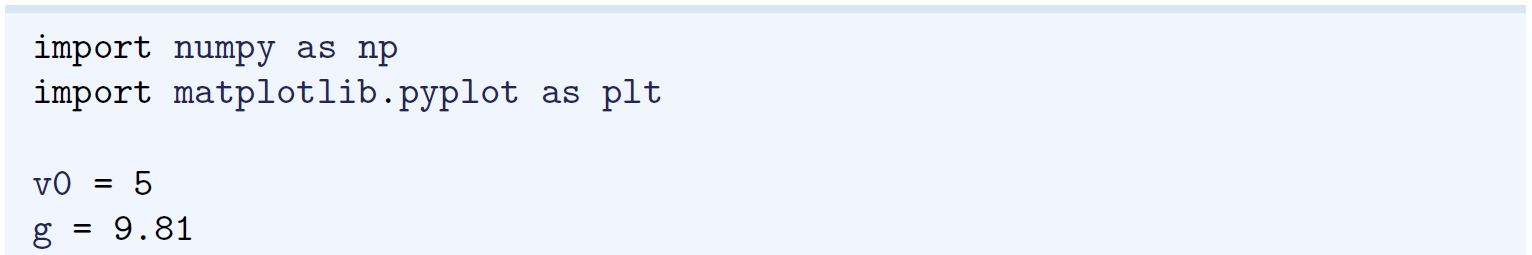
\includegraphics[width=0.9\textwidth]{figures/LLp19}
	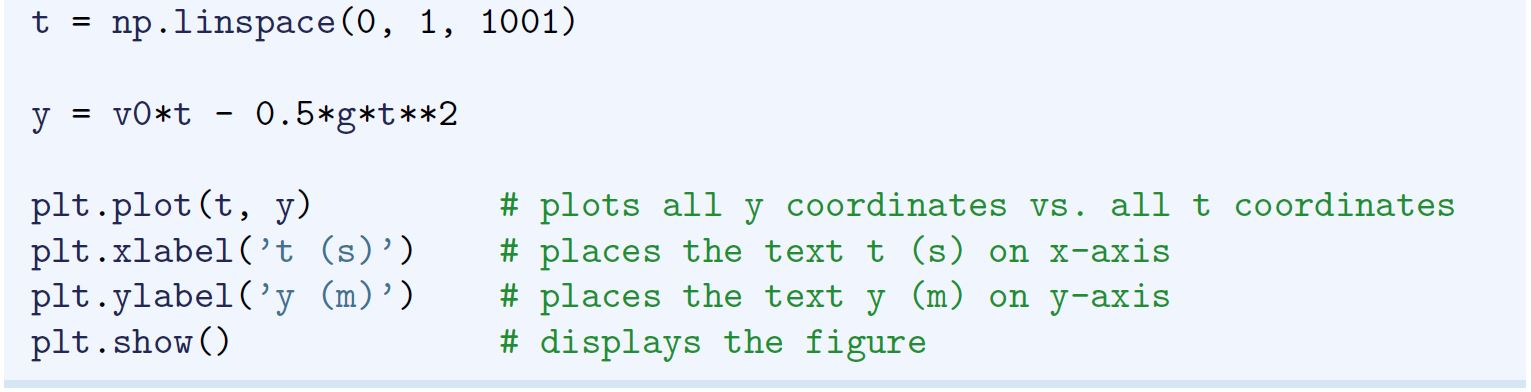
\includegraphics[width=0.9\textwidth]{figures/LLp20a}
\end{figure}
\vspace*{-8mm}
\begin{itemize}
\item \texttt{linspace} function and our first \red{\emph{array}}
\item \red{\emph{vectorisation}} in \texttt{y = v0*t - 0.5*g*t**2}
\item plot commands
\end{itemize}

\end{frame}

%==============================================================

\begin{frame}[fragile]
\frametitle{Program output}
When we run \texttt{ball\_plot.py} in PyCharm:
\begin{figure}[ht]
	\centering
	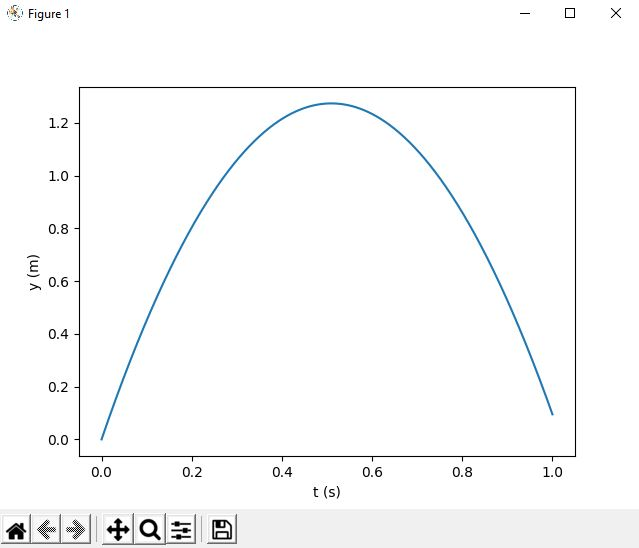
\includegraphics[width=0.6\textwidth]{figures/LLp20output}
\end{figure}

\end{frame}

%==============================================================

\begin{frame}[fragile]
\frametitle{Our first array}

\begin{figure}[ht]
	\centering
	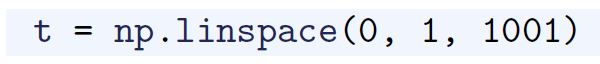
\includegraphics[width=0.9\textwidth]{figures/LLp20b}
\end{figure}
\vspace*{-8mm}
\begin{itemize}
\item creates $1001$ coordinates on the interval $[0,1]$:
\item[] $0, 0.001, 0.002, \ldots, 1$
\item Python stores these as an \red{\emph{array}}
\item think of the array \texttt{t} as a collection of ``boxes'' in computer memory
\item Python numbers these boxes consecutively from zero upwards:
\item[] \texttt{t[0], t[1], t[2], \ldots, t[1000]}
\end{itemize}

%The linspace Function Next, there is a call to the function linspace from the
%numpy library. When n evenly spaced floating point numbers are sought on an
%interval [a, b], linspace may generally be called like this:
%np.linspace(a, b, n)
%This means that the call
%t = np.linspace(0, 1, 1001)
%creates 1001 coordinates between 0 and 1, inclusive at both ends. The mathematically
%inclined reader might agree that 1001 coordinates correspond to 1000 equal
%sized intervals in [0, 1] and that the coordinates are then given by ti = 1−0
%1000 i = i
%1000 ,
%i = 0, 1, . . . , 1000.
%The object returned from linspace is an array, i.e., a certain collection of (in
%this case) numbers. Through the assignment, this array gets the name t. If we like,
%we may think of the array t as a collection of “boxes” in computer memory (each
%containing a number) that collectively go by the name t (later, we will demonstrate
%how these boxes are numbered consecutively from zero and upwards, so that each
%“box” may be identified and used individually).

\end{frame}

%==============================================================

\begin{frame}[fragile]
\frametitle{Vectorization}

\vspace*{-4mm}
\begin{figure}[ht]
	\centering
	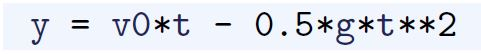
\includegraphics[width=0.6\textwidth]{figures/LLp21a}
\end{figure}
\vspace*{-4mm}

\begin{itemize}
	\item right-hand side is computed for every entry in the array \texttt{t}
	\item ie: for \texttt{t[0], t[1], t[2], \ldots, t[1000]}
	\item[\green{\cmark}] yields a collection of 1001 numbers in the result \texttt{y}, which
	(automatically) also becomes an array!
	\item technique of computing all numbers ``in one chunk'' is called \red{\emph{vectorization}}
\end{itemize}

\end{frame}

%==============================================================

\begin{frame}[fragile]
\frametitle{Plotting commands}

Plotting commands are new, but simple:

\begin{figure}[ht]
	\centering
	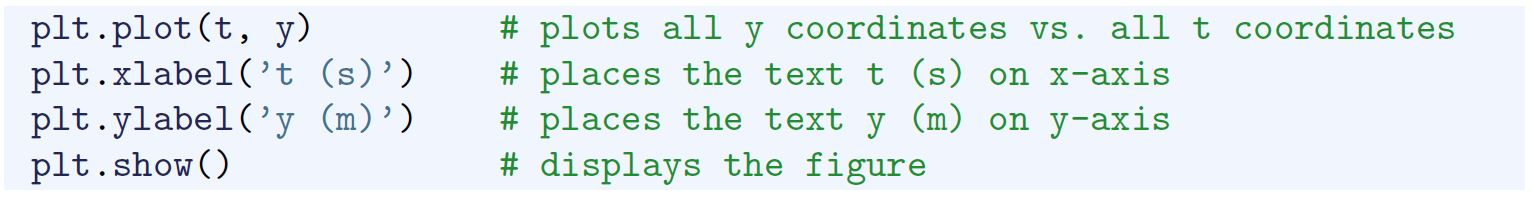
\includegraphics[width=\textwidth]{figures/LLp21b}
\end{figure}

\end{frame}

%==============================================================

\begin{frame}[fragile]
\frametitle{Live demo of simple plotting}

\end{frame}

%==============================================================

\begin{frame}[fragile]
\frametitle{4) Plotting, printing and input data}

\begin{itemize}
\item \texttt{Matplotlib} is standard plotting package in Python
\item have already seen array \texttt{y} (heights) plotted against another array \texttt{t} (points in time) 
\end{itemize}
\vspace*{-6mm}
\begin{center}
{\small\blue{
\textbf{
\texttt{plt.plot(t,y)}}}
}
\end{center}
\vspace*{-8mm}
\begin{figure}[ht]
	\centering
	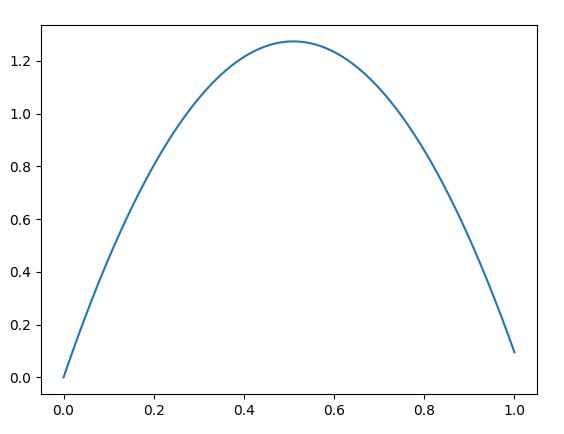
\includegraphics[width=0.4\textwidth]{figures/LLp22a}
\end{figure}

\end{frame}

%==============================================================

\begin{frame}[fragile]
\frametitle{Line styles}

\begin{figure}[ht]
	\centering
	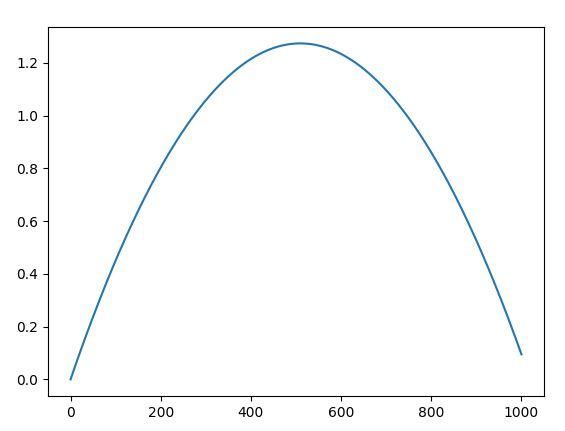
\includegraphics[width=0.5\textwidth]{figures/LLp23aoutput}%
	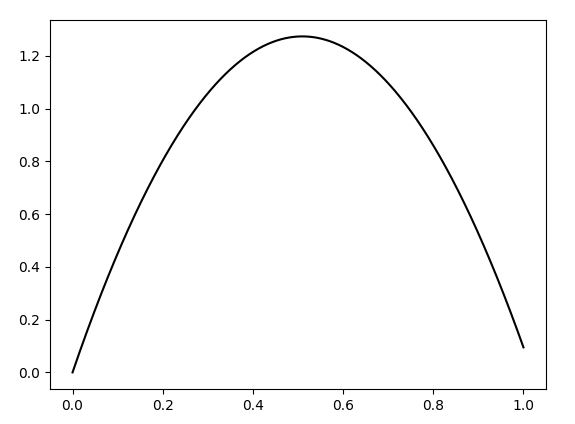
\includegraphics[width=0.5\textwidth]{figures/LLp23boutput}
\end{figure}
\vspace*{-8mm}
\begin{itemize}
\item[left:] \texttt{plt.plot(y) \# x-axis indices}
\item[right:] \texttt{plt.plot(t, y, 'k')  \# black line}
\end{itemize}

\end{frame}

%==============================================================

\begin{frame}[fragile]
\frametitle{More line styles}

\begin{figure}[ht]
	\centering
	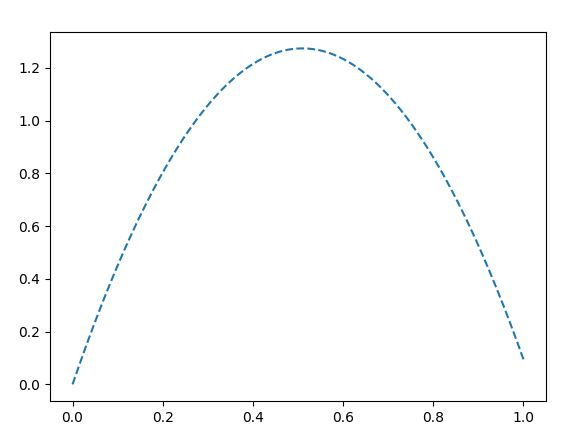
\includegraphics[width=0.5\textwidth]{figures/LLp23coutput}%
	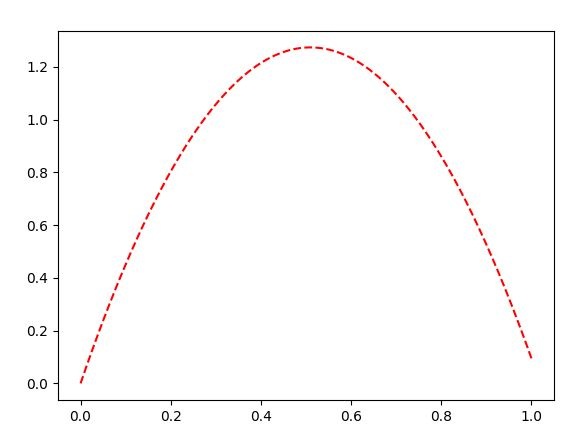
\includegraphics[width=0.5\textwidth]{figures/LLp23doutput}
\end{figure}
\vspace*{-8mm}
\begin{itemize}
\item[left:] \texttt{plt.plot(t, y, '--') \# dashed}
\item[right:] \texttt{plt.plot(t, y, 'r--') \# red dashed}
\end{itemize}

\end{frame}

%==============================================================

\begin{frame}[fragile]
\frametitle{Plotting points only}

\begin{figure}[ht]
	\centering
	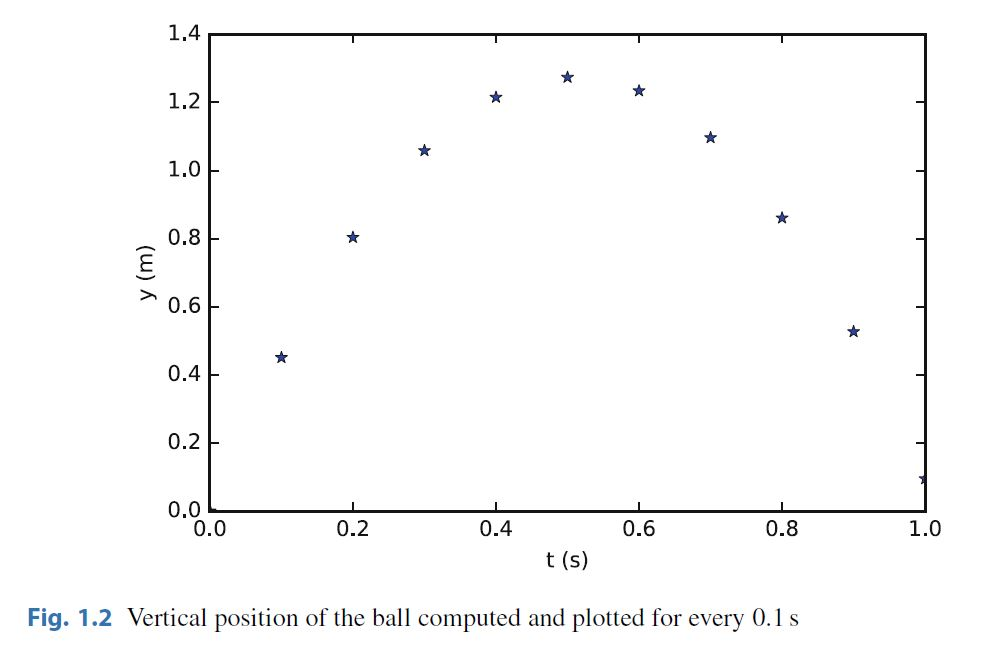
\includegraphics[width=0.7\textwidth]{figures/LLp24a}
	
\includegraphics[width=\textwidth]{figures/LLp23a}
	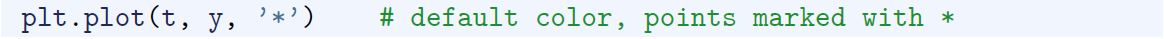
\includegraphics[width=\textwidth]{figures/LLp23b}
\end{figure}

\end{frame}

%==============================================================

\begin{frame}[fragile]
\frametitle{Decorating a plot}

\vspace*{-3mm}
\begin{figure}[ht]
	\centering
	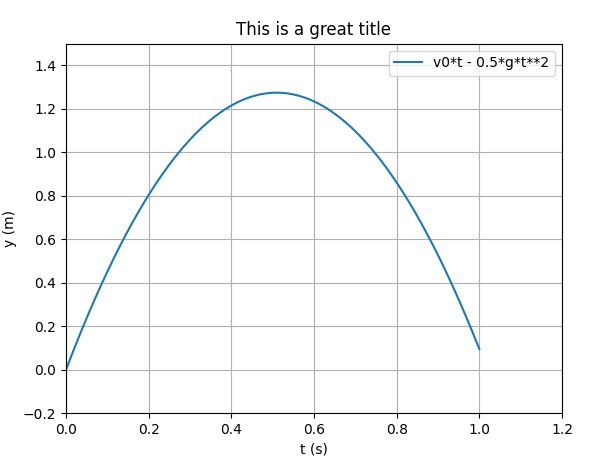
\includegraphics[width=0.8\textwidth]{figures/LLp24output}
\end{figure}

\end{frame}

%==============================================================

\begin{frame}[fragile]
\frametitle{Decorating a plot}

\begin{itemize}
\item add a legend
\vspace*{-5mm}
\begin{figure}[ht]
	\centering
	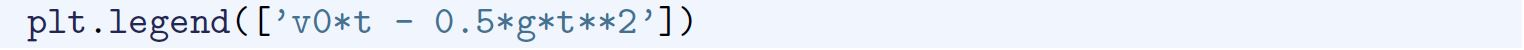
\includegraphics[width=\textwidth]{figures/LLp24c}
\end{figure}

\item add a grid
\vspace*{-5mm}
\begin{figure}[ht]
	\centering
	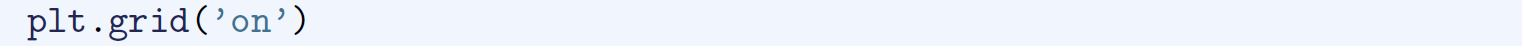
\includegraphics[width=\textwidth]{figures/LLp24d}
\end{figure}
\item display a title
\vspace*{-5mm}
\begin{figure}[ht]
	\centering
	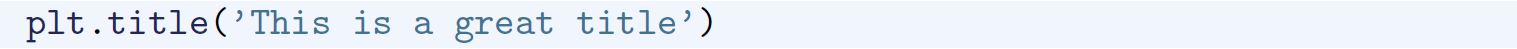
\includegraphics[width=\textwidth]{figures/LLp24e}
\end{figure}
\item override default ranges for plot axes
\vspace*{-5mm}
\begin{figure}[ht]
	\centering
	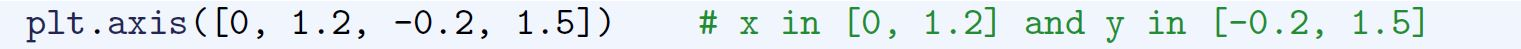
\includegraphics[width=\textwidth]{figures/LLp24f}
\end{figure}
\end{itemize}

\end{frame}

%==============================================================

\begin{frame}[fragile]
\frametitle{Multiple curves in the same plot}

\begin{figure}[ht]
	\centering
	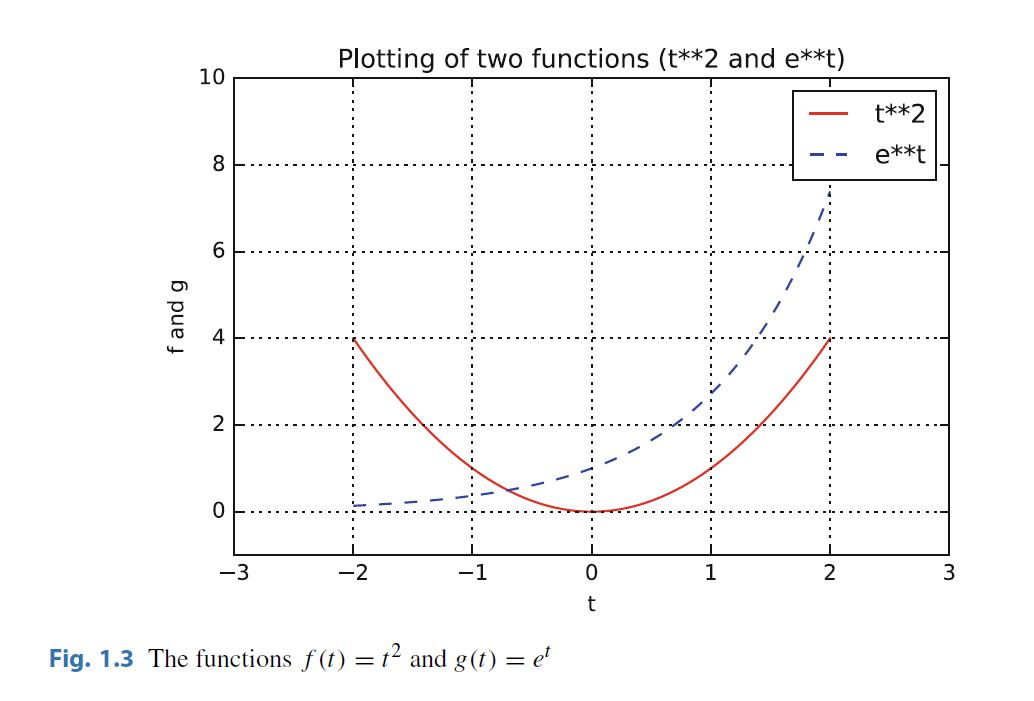
\includegraphics[width=0.9\textwidth]{figures/LLp25b}
\end{figure}

\end{frame}

%==============================================================

\begin{frame}[fragile]
\frametitle{Multiple curves in the same plot}

\vspace*{-3mm}
\begin{figure}[ht]
	\centering
	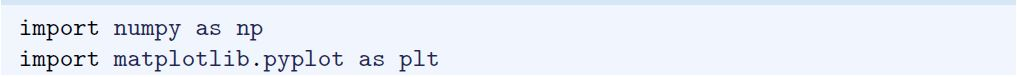
\includegraphics[width=0.9\textwidth]{figures/LLp24b}
	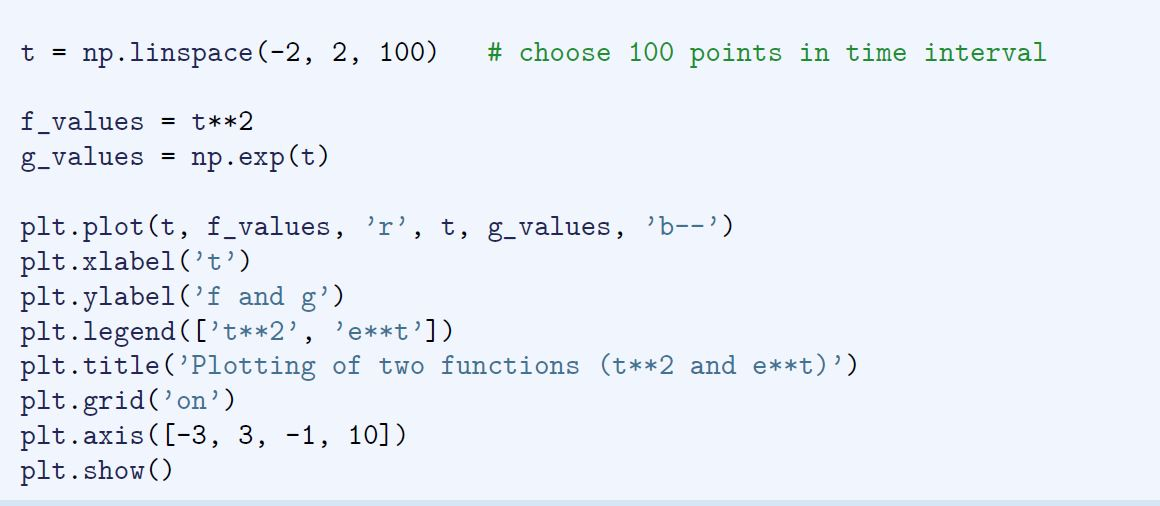
\includegraphics[width=0.9\textwidth]{figures/LLp25a}
\end{figure}
\vspace*{-3mm}
Key line of code for multiple curves:
\begin{figure}[ht]
	\centering
	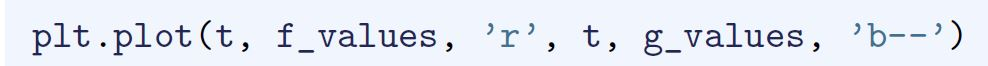
\includegraphics[width=0.7\textwidth]{figures/LLp25c}
\end{figure}

\end{frame}

%==============================================================

\begin{frame}[fragile]
\frametitle{Printing variables and strings}

\begin{itemize}
\item print the value of variable \texttt{y}

\begin{figure}[ht]
	\centering
	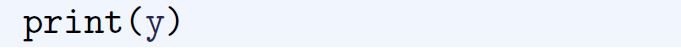
\includegraphics[width=0.8\textwidth]{figures/LLp27a}
\end{figure}

\vspace*{10mm}
\item print the string \texttt{This is some text}
\begin{figure}[ht]
	\centering
	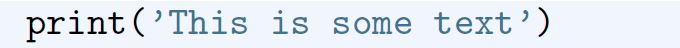
\includegraphics[width=0.8\textwidth]{figures/LLp27b}
\end{figure}
	\begin{itemize}
		\item enclose text in single quotes
	\end{itemize}
\end{itemize}

\end{frame}

%==============================================================

\begin{frame}[fragile]
\frametitle{Print \emph{one} variable and text combined}

\begin{itemize}
\item if variable \texttt{v1} has value $10.0$ and you want to display as follows:

\begin{figure}[ht]
	\centering
	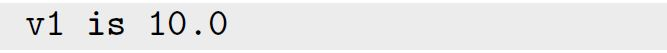
\includegraphics[width=0.8\textwidth]{figures/LLp28a}
\end{figure}

%\vspace*{5mm}
\item use the following Python code:
\begin{figure}[ht]
	\centering
	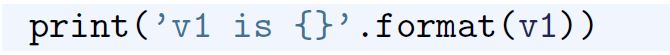
\includegraphics[width=0.8\textwidth]{figures/LLp28b}
\end{figure}
	\begin{itemize}
		\item pair of curly brackets \{\} acts as a \red{\emph{placeholder}}
		\item \ldots says \emph{where} to place value
		\item \texttt{.format(v1)} converts variable \texttt{v1} to string \texttt{10.0}
	\end{itemize}
\end{itemize}

\end{frame}

%==============================================================

\begin{frame}[fragile]
\frametitle{Printing \emph{several} variables and text combined}

\begin{itemize}
\item if \texttt{v1} and \texttt{v2} have values $10.0$ and $20.0$ and you want to display as follows:

\begin{figure}[ht]
	\centering
	
\includegraphics[width=0.8\textwidth]{figures/LLp28d}
\end{figure}

\item use the following Python code:
\begin{figure}[ht]
	\centering
	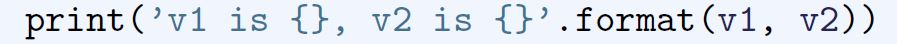
\includegraphics[width=0.8\textwidth]{figures/LLp28c}
\end{figure}
\vspace*{-3mm}
	\begin{itemize}
		\item now \emph{two} pairs of curly brackets \{\} act as a placeholders
		\item \texttt{.format(v1,v2)} dictates the order in which placeholders are filled
		\item in this case: \texttt{v1} first, then \texttt{v2}
	\end{itemize}
\end{itemize}

\end{frame}

%==============================================================

\begin{frame}[fragile]

\frametitle{Controlled printing: decimals, scientific notation \& strings}

\begin{itemize}
\item[] 	\begin{itemize}
		\item real number $12.89643$
		\item integer $42$
		\item string \texttt{some message}
	\end{itemize}

\item supose you want to display as follows:
\begin{figure}[ht]
	\centering
	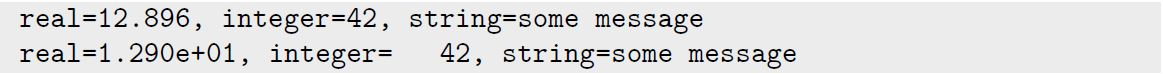
\includegraphics[width=0.8\textwidth]{figures/LLp29a}
\end{figure}

\item use the following Python code:
\begin{figure}[ht]
	\centering
	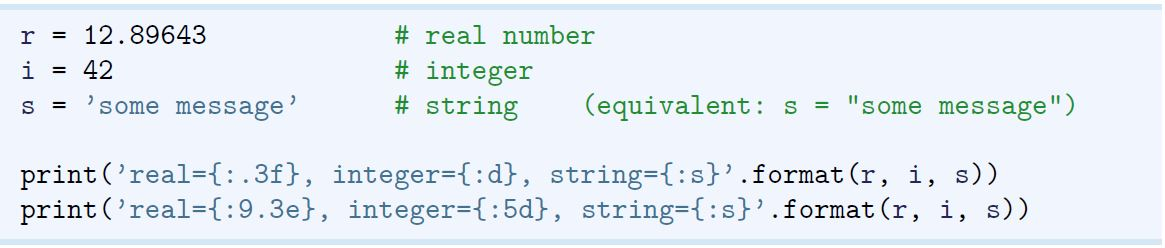
\includegraphics[width=0.8\textwidth]{figures/LLp29b}
\end{figure}

\end{itemize}

\end{frame}

%==============================================================

\begin{frame}[fragile]

\frametitle{Controlled printing: decimals, scientific notation \& strings}

\begin{itemize}
\item first call to \texttt{print}

\begin{figure}[ht]
	\centering
	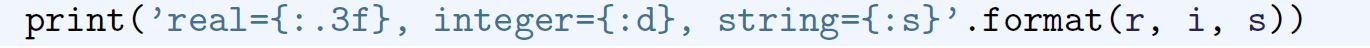
\includegraphics[width=0.9\textwidth]{figures/LLp30a}
\end{figure}
\vspace*{-3mm}
	\begin{itemize}
		\item \texttt{:.3f} \quad write number \texttt{r} compactly using 3 decimals
		\item \texttt{:d} \quad~~~ write integer \texttt{i} as compactly as possible
		\item \texttt{:s} \quad\quad~\!\! write string \texttt{s}
	\end{itemize}
	
\item second call to \texttt{print}
\begin{figure}[ht]
	\centering
	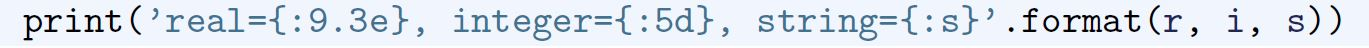
\includegraphics[width=0.9\textwidth]{figures/LLp30b}
\end{figure}
\vspace*{-3mm}
	\begin{itemize}
		\item \texttt{:9.3e} \quad write number \texttt{r} in \red{\emph{scientific notation}} with \\
		\qquad\qquad\qquad $3$ decimals in field of width $9$ characters
		\item \texttt{:5d} \quad~~~ write integer \texttt{i} in field of width $5$ characters
	\end{itemize}
\end{itemize}

\end{frame}

%==============================================================

\begin{frame}[fragile]
\frametitle{Live demo of plotting and printing}

\end{frame}

\end{document}
